\begin{figure}[h]
    \centering
    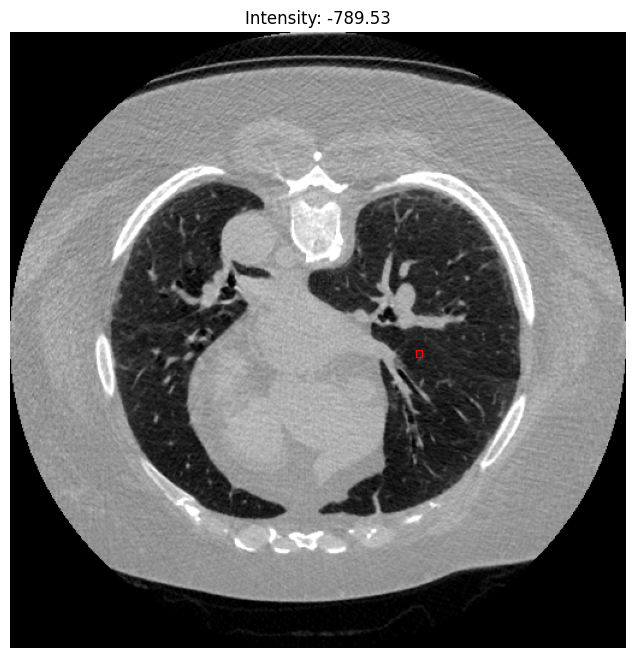
\includegraphics[width=0.6\linewidth]{images/non-visible-nodule-1.png}
    \caption{Example of a slice with an annotated nodule (at the indicated depth) that does not contain any visible tissue from the nodule itself. At the top the mean intensity expressed in Hounsfield Units (HU) of the area within the annotation. }
    \label{fig:non-visible-nodule}
\end{figure}